\subsection{HDMI Output Protocol}

The standard PYNQ video overlay drives the display through a
\textit{Video Direct Memory Access} (VDMA) engine: the PS renders a
complete frame into a DDR3 framebuffer, the VDMA DMA-transfers it into
an AXI4-Stream, and a \textit{Video Timing Controller} (VTC) clocks it
through \textit{AXI4-Stream to Video Out} and \textit{RGB-to-DVI} to
the HDMI port. Every pixel therefore traverses the PS $\rightarrow$
DDR $\rightarrow$ PL path before reaching the display.

\vspace{0.5em}

This architecture is incompatible with a free-running hardware
raycaster. The VDMA expects a complete, PS-written framebuffer before
each transfer, the DDA engine produces pixels \textit{in column order
at PL clock rate}, with no ARM involvement. Inserting a framebuffer
would require the PS to stall the raycaster, copy $320 \times 240
\times 3 = \mathbf{225\,\text{kB}}$ to DDR, and signal the VDMA,
adding one full frame of latency ($\sim$16.7\,ms at 60\,fps) and
consuming AXI bandwidth that is shared with the network stack.

\vspace{0.5em}

Instead, the raycaster AXI-Stream is connected directly to
\texttt{v\_axi4s\_vid\_out\_0}, with the VTC providing the pixel clock
and sync signals and the RGB-to-DVI IP serialising the output to TMDS,
as shown in Figure~\ref{fig:hdmi-block}. The VDMA is removed entirely.
Pixels flow raycaster $\rightarrow$ AXI-Stream $\rightarrow$ Video Out
$\rightarrow$ TMDS without any intermediate memory transaction.

\begin{figure}[H]
    \centering
    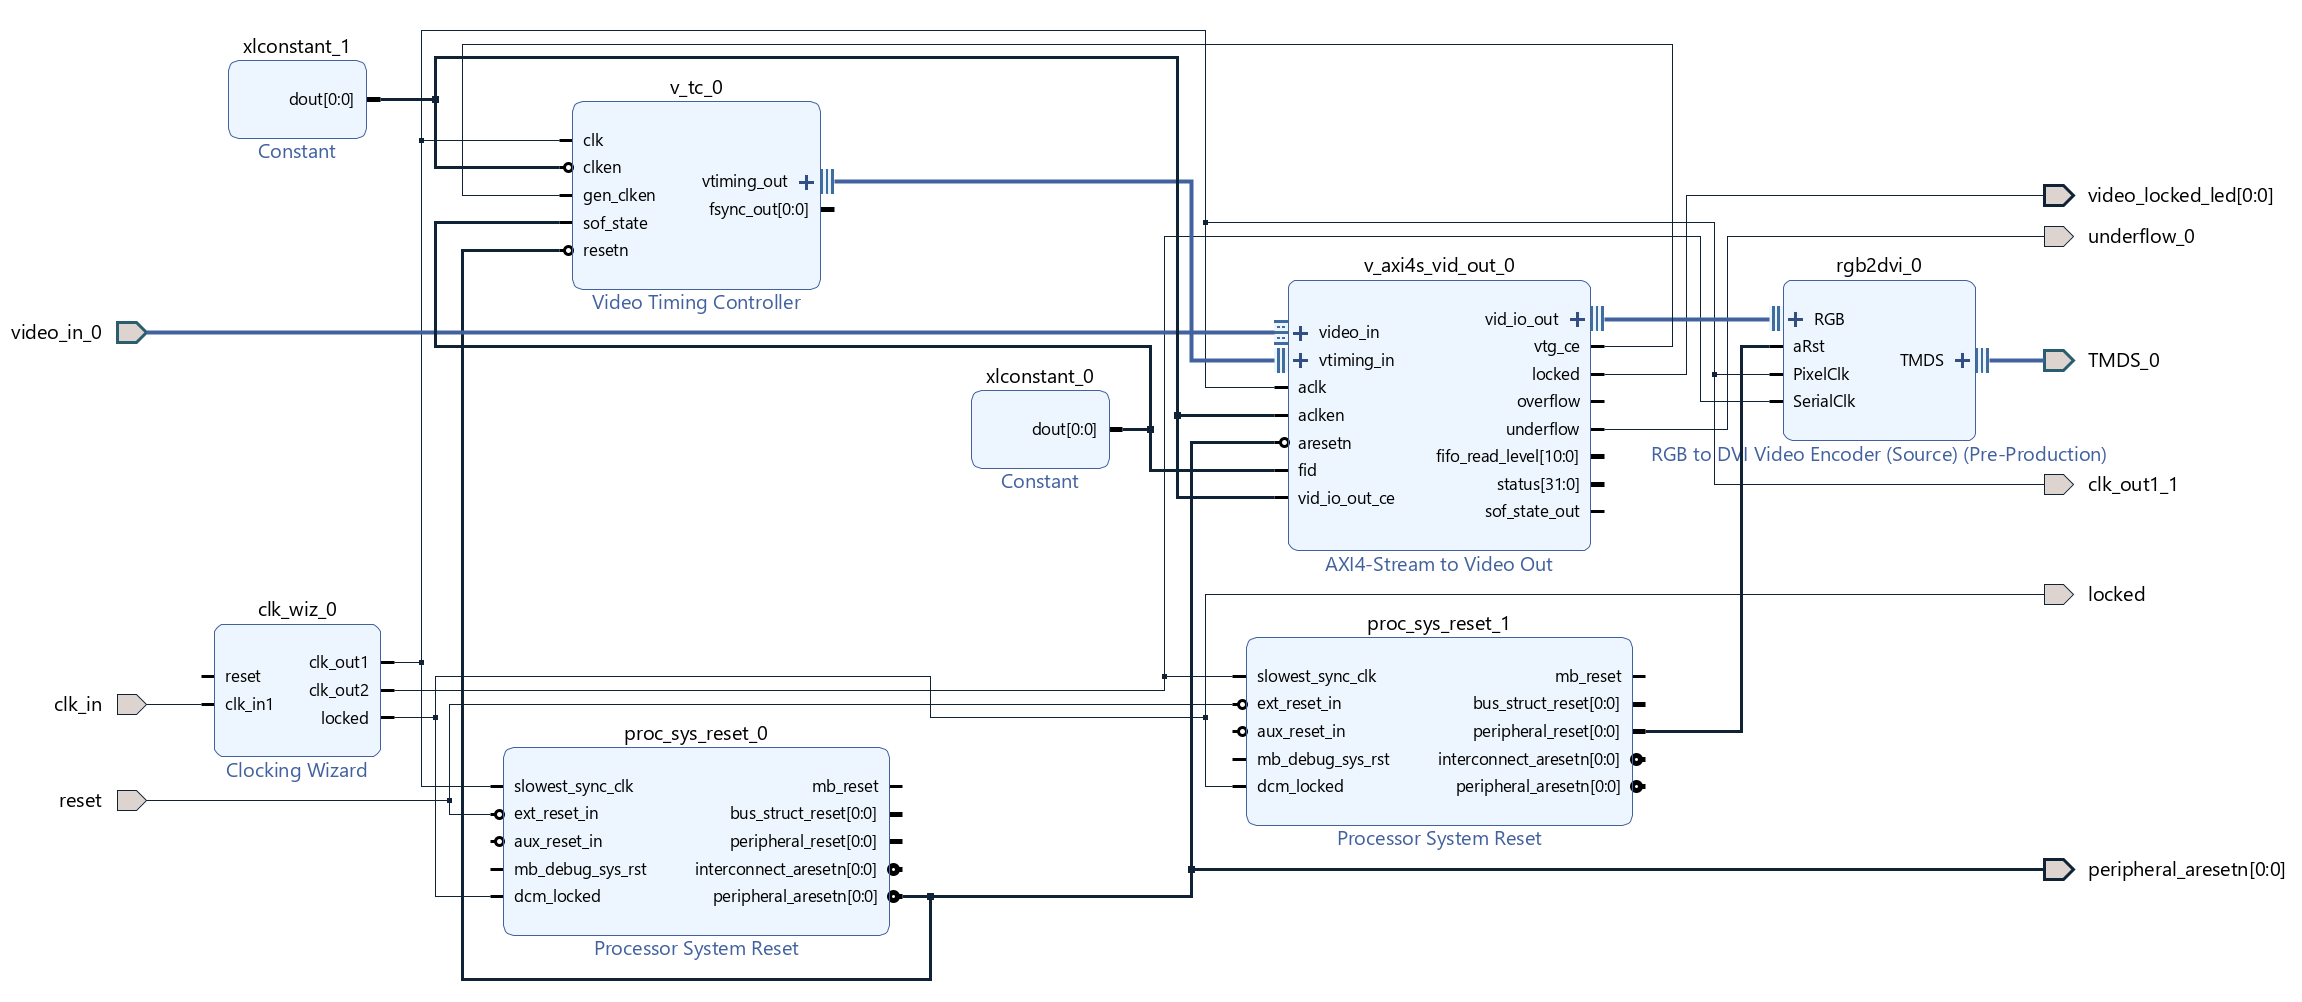
\includegraphics[width=\columnwidth]{images/vivado_hdmi_block.png}
    \caption{VDMA-free video pipeline: raycaster pixel stream feeds
             directly into AXI4-Stream to Video Out, bypassing DDR.}
    \label{fig:hdmi-block}
\end{figure}

The hardware consequences of removing the VDMA are:

\begin{itemize}
    \item \textbf{Latency:} End-to-end pixel latency drops from one
    full frame ($\sim$16.7\,ms) to the AXI handshake delay
    ($<1\,\mu$s)

    \item \textbf{AXI bandwidth:} The DDR bus is no longer saturated
    by display transfers. At 60\,fps the VDMA would consume
    $225\,\text{kB} \times 60 \approx \mathbf{13\,\text{MB/s}}$ of
    AXI bandwidth; this is now fully available to the PS for UDP
    packet handling and game-state writes to BRAM.

    \item \textbf{PS load:} The ARM core is relieved of all DMA
    descriptor management and framebuffer allocation. The game loop
    writes only a 34-byte state packet to BRAM each tickrather than a full rendered frame.
\end{itemize} 

The two \texttt{proc\_sys\_reset} instances and the \textit{Clocking
Wizard} remain from the original pipeline to manage the AXI and pixel
clock domains correctly, no additional clock-domain crossings were
introduced.

\paragraph{Resource cost:}
The VDMA-free pipeline consumes no additional BRAM or LUTs relative to
the stock Xilinx video stack, the savings are in DDR bandwidth and PS
cycles rather than PL fabric. The VTC, AXI4S-to-Video-Out, and
RGB-to-DVI IPs retain their original footprint
($\sim$1\,800 LUTs, 0 BRAM tiles for the video path alone).